% -----------------------------------------------
% Template for JIM
%     jim.sty -> style file
% By Eloi Batlle (eloi@iua.upf.es), changes for 
% ICMC by Bram de Jong (bdejong@iua.upf.es)
% changes for JIM 2007 by Dominique Fober (fober@grame.fr)
% changes for JIM 2009 by Olivier Tache (olivier.tache@imag.fr)
% -----------------------------------------------

\documentclass{article}
\usepackage{jim,amsmath}
\usepackage[utf8]{inputenc}
\usepackage[francais]{babel}
\usepackage[T1]{fontenc}
%\usepackage{pxfonts}
\usepackage{graphicx}
\usepackage{balance}
\usepackage{ifpdf}

\usepackage{verbatim}
\usepackage{color}
\usepackage{textcomp}

\definecolor{mygrey}{gray}{0.93}
\definecolor{figOrange}{RGB}{212,85,0}
\definecolor{figRed}{RGB}{128,0,0}
\definecolor{red}{RGB}{250,0,0}
\definecolor{figBlue}{RGB}{0,136,170}

\newenvironment{ExprCode}		{\vspace{-2mm} \small\verbatim}{\endverbatim\vspace{-2mm}}
\newcommand{\OSC}[1]{\texttt{#1}}
\newcommand{\oper}[1]{\textcolor{figRed}{#1}}
\newcommand{\param}[1]{\textcolor{figOrange}{#1}}
\newcommand{\prefix}[1]{\textcolor{figBlue}{#1}}

\newcommand{\note}[1]{\textcolor{red}{(#1)}}


\newcommand{\sExpr}{\emph{score expressions}}
\newcommand{\SExpr}{\emph{Score expressions}}
\newcommand{\lowTilde}{\texttildelow}
\newcommand{\tab}{\hspace*{4mm}}

\let\olditemize\itemize
\let\oldenditemize\enditemize
\renewenvironment{itemize} 	{\olditemize \setlength{\itemsep}{1mm}}{\oldenditemize}

\newcommand{\sample}	[1]			{\vspace{-0.2em}\begin{center}\colorbox{mygrey}{\begin{minipage}[t]{0.95\columnwidth} {\small \texttt{#1}}\end{minipage}}\end{center}}


% Title.
% ------
\title{Composition de partitions symboliques dnas INScore}

% Single \textsc{address}
% To use with only one author or several with the same address
% ---------------
\oneauthor
  {G. Lepetit-Aimon \qquad D. Fober \qquad Y. Orlarey \qquad S. Letz} {Grame \\
  Centre nationale de création musicale \\
  Lyon - France \\
     {\tt {\small \{gabriel.lepetit.aimon,fober,orlarey,letz\}@grame.fr}}}

% Two addresses
% --------------
%\twoauthors
%  {First author} {School \\ Department}
%  {Second author} {Company \\ Address}

% Three addresses
% --------------
%\threeauthors
%  {Auteur 1} {Organisme \\ Adresse électronique}
%  {Auteur 2} {Organisme \\ Adresse électronique}
%  {Auteur 3} {Organisme \\ Adresse électronique}

\begin{document}
%
\maketitle
%
\begin{abstract}
INScore est un environnement pour le design de partition interactives augmentées, tourné vers des usages non conventionnels de la notation musicale. L'environnement permet d'utiliser et de composer des ressources graphiques arbitraires pour la représentation de la musique aussi bien que de la notation symbolique aux formats GMN (Guido Music Notation) ou MusicXML. INScore a été étendu pour fournir des opérations de composition de partitions en notation symbolique avec un jeu d'opérateurs qui de manière consistante, prennent des partitions en entrée pour produire une partition en sortie. L'API d'INScore inclus des \sExpr , aussi bien au niveau OSC que dans son langage de script. 
Le travail présenté est basé sur une recherche précédente qui a porté sur les problèmes de consistance de la notation musicale à travers des opérations de composition de partitions. Ce sont les aspects langage et stratégies d'évaluation des \SExpr\ qui sont abordés ici.
\end{abstract}

%==============================================================
\section{Introduction}\label{sec:introduction}

Contemporary music creation poses numerous challenges to the music notation. Spatialized music, new instruments, gesture based interactions, real-time and interactive scores, are among the new domains that are now commonly explored by artists. 
Classical music notation doesn't cover the needs of these new musical forms and numerous research and approaches have recently emerged, testifying to the maturity of the music notation domain, in the light of computer tools for music notation and representation.
Issues like writing spatialized music \cite{Ellberger_tenor2015}, addressing new instruments \cite{tmays:2014} or new interfaces \cite{kschlei:2015} (to cite just a few), are now subject of active research and proposals.

Interactive music and real-time scores are also representative of an expanding domain in the music creation field. The advent of the digital score and the maturation of the computer tools for music notation and representation constitute the basement for the development of this musical form, which is often grounded on non-traditional music representation \cite{RSmith_tenor2015} \cite{Hope_tenor2015} but may also use the common music notation \cite{Hoadley12,hoadley14}. 

In order to address the notation challenges mentionned above, INScore \cite{Fober:12a,fober14c} has been designed as an environment opened to non-conventional music representation (although it supports symbolic notation), and turned to real-time and interactive use \cite{Fober:13b, Fober:14b}. It is clearly focused on music representation only and in this way, differs from tools integrated into programming environments like Bach \cite{agostini12b} or MaxScore \cite{didko08}. 

INScore has been extended with \sExpr\ that provide symbolic scores composition features (e.g., putting scores in sequence or in parallel). Building new scores from existing scores at symbolic  level is not new. Haskell is providing such features \cite{Quick:2013:GAM:2505341.2505345}. Freeman and Lee proposed score composition operations in a real-time and interactive notation context \cite{Lee:2013}. Regarding the score operations used by INScore, they are imported from a previous work \cite{fober12b} that was focusing on the music notation consistency through arbitrary composition. 

The novelty of the proposed approach relies on the dynamic aspects of the scores composition operations, as well as on the persistence of the score expressions. A score may be composed as an arbitrary graph of score expressions and equipped with a fine control over the changes propagation.

The paper introduces first the score composition expressions. Next, the different evaluation strategies are explained and illustrated with examples. The articulation with the INScore environment is presented in detail and followed by concrete use cases. An extension of the primary scores composition design to \sExpr\ composition is next introduced. A generalization of this approach to the whole set of INScore graphic objects is finally considered in the concluding section.  



%==============================================================
\section{Taille de la page}\label{sec:page_size}

Les actes seront imprimés au format A4 (21 x 29.7 cm). Le contenu de chaque page doit pouvoir tenir dans un rectangle de (17 x 24.7 cm) centré sur la page, commençant à 2 cm du haut de la page et s'arrêtant à  3 cm du bas de la page. Les marges gauche et droite doivent être de 2 cm. Le texte est présenté sur deux colonnes (8,1cm) avec une gouttière  de 0,8 cm. Le texte doit être justifié à gauche et à droite.

\section{Police de caracteres}\label{sec:typeset_text}

\subsection{Corps du texte}\label{subsec:body}

Utiliser la police Times 10 pt (points). N'utiliser une police sans serif ou non proportionnelle que pour des raisons particulières, par exemple pour distinguer des lignes de code du reste du texte.

\subsection{Titre et auteurs}

Le titre est en Times 14 pt, gras, majuscule, centré. Les noms des auteurs sont centrés. Si l'adresse est la même pour tous les auteurs, elle ne doit figurer qu'une seule fois, centrée. Dans le cas contraire, elle doit apparaître sous le nom de chaque auteur.

\subsection{Numéro de page, haut de page et  bas de page}

Ne pas inclure  de numéro de page, de haut de page ou de bas de page lors de votre soumission. Ils seront ajoutés par l'éditeur.

\section{Sections}

Les titres de sections sont en Times, 10 pt gras, centrés avec 1 ligne d'espace au-dessus du titre de section, et 1/2 espace au-dessous. Pour un titre de section immédiatement suivi d'un titre de sous-section, ne pas additionner les deux espaces.

\subsection{Sous-sections}

Les titres de sous-sections sont en Times 10 pt alignés à gauche, avec une ligne d'espace au-dessus, et 1/2 ligne d'espace au-dessous.

\subsubsection{Sous-sous-sections}

Les sous-sous-sections sont en Times 10 pt italique, alignés à gauche, avec 1 ligne d'espace au-dessus et 1/2 ligne d'espace au-dessous.

On évitera d'utiliser plus de trois niveaux de section.


\section{Notes de bas de page et Figures}

\subsection{Notes de bas de page}

Indiquer la note de bas de page avec un numéro dans le texte\footnote{Ceci est une note de bas de page}.  Utiliser la police Times 8 pt. Placer les notes en bas de chaque page où elles vont apparaitre. Faire précéder la note d'une ligne horizontale de 0,5 pt.

\subsection{Illustrations, figures et tableaux}

Toutes les illustrations devront être centrées dans une colonne, propres et lisibles (Figure 1). L'impression des actes sera en noir et blanc. Les figures doivent donc faire sens en noir et blanc. Les numéros de figure, de tableau et leur légende doivent toujours apparaître en dessous de la figure. Laisser une ligne d'espace entre la figure et sa légende. Chaque figure ou tableau est numéroté consécutivement. Les légendes seront présentées en Times 10 pt et indentées. Placer les illustrations aussi près des références que possible. Elles peuvent être placées au centre de la page, traversant les deux colonnes, dans une limite de 17cm.

\begin{table}
\begin{center}
\begin{tabular}{|l|l|}
\hline
Texte & Valeur \\
\hline
hello jim  & 1073 \\
\hline
\end{tabular}
\end{center}
\caption{La légende du tableau devra être placée sous le tableau.}
\label{tab:example}
\end{table}

%\begin{figure}
%\centerline{\framebox{
%	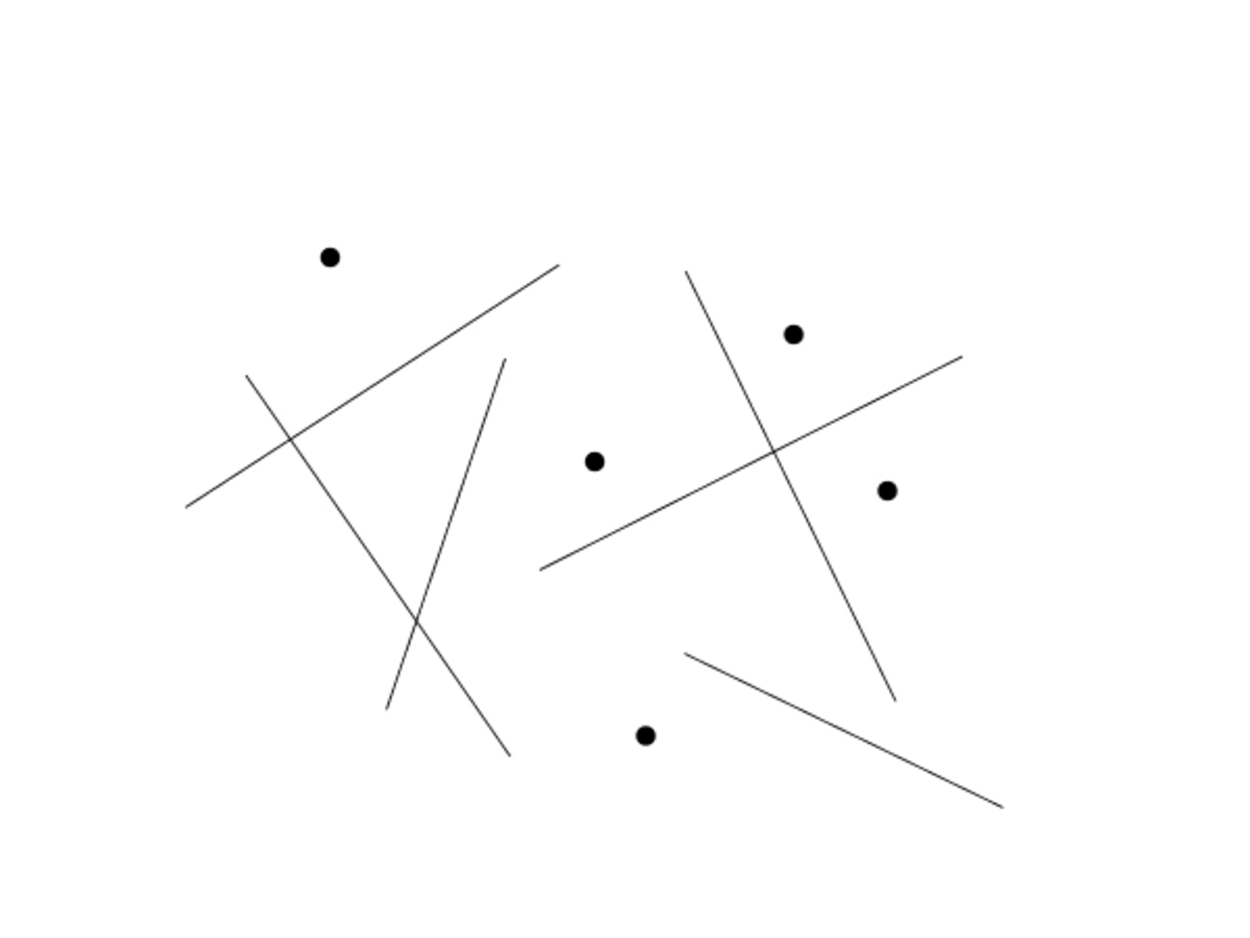
\includegraphics[width=\columnwidth]{figure}}}
%\caption{La légende de la figure devra être placée sous la figure.}
%\label{fig:example}
%\end{figure}

\section{Equations}

Les équations devront être placées sur des lignes séparées et numérotées. Le numéro devra être placé à droite.

\begin{equation}
E=mc^{2}
\end{equation}

\section{Citations}

Toutes les références bibliographiques des citations devront être listées dans la section "\textsc{References}", numérotées et en ordre alphabétique. Toutes les références  listées devront être citées dans le texte. Quand  vous vous référez au document dans le texte, précisez son numéro \cite{Author:00}.

%\balance
\bibliography{../interlude}

\end{document}
